% Master layout: compiled at A0, then proportionally reduced to the required
% A1 portrait submission size by poster/Makefile.
\documentclass[final]{beamer}

\usepackage[orientation=portrait,size=a0,scale=1.18]{beamerposter}
\usetheme{gemini}
\usecolortheme{nott}
\usepackage{graphicx}
\usepackage{booktabs}
\usepackage{tabularx}
\usepackage{ragged2e}
\usepackage[most]{tcolorbox}
\usepackage{hyperref}
\graphicspath{{../docs/figures/week06/}}

\newlength{\sepwidth}
\newlength{\colwidth}
\setlength{\sepwidth}{0.022\paperwidth}
\setlength{\colwidth}{0.467\paperwidth}
\newcommand{\separatorcolumn}{\begin{column}{\sepwidth}\end{column}}

\definecolor{accentblue}{RGB}{37,104,153}
\definecolor{pale}{RGB}{241,246,250}
\definecolor{warm}{RGB}{247,241,230}

\newtcolorbox{posterbox}[1]{
  enhanced,
  colback=white,
  colframe=nottblue,
  coltitle=white,
  colbacktitle=nottblue,
  fonttitle=\bfseries\fontsize{37}{44}\selectfont,
  title={\centering #1},
  boxrule=2.2pt,
  arc=0mm,
  top=13pt,bottom=13pt,left=18pt,right=18pt,
  toptitle=10pt,bottomtitle=10pt,
  before skip=0pt,after skip=18pt
}

\newtcolorbox{takeaway}{
  enhanced,colback=pale,colframe=accentblue,boxrule=2.2pt,arc=2mm,
  top=14pt,bottom=14pt,left=18pt,right=18pt
}

\newtcolorbox{finalbox}{
  enhanced,colback=nottblue,colframe=nottblue,coltext=white,
  boxrule=0pt,arc=0mm,height=8.2cm,valign=center,
  top=20pt,bottom=20pt,left=24pt,right=24pt
}

\newcommand{\metric}[2]{%
  \begin{minipage}[c][4.8cm][c]{0.30\linewidth}
    \centering{\fontsize{43}{48}\selectfont\bfseries\color{accentblue}#1}\par
    \vspace{0.25cm}{\fontsize{20}{25}\selectfont #2}
  \end{minipage}}

\title{}
\author{}
\institute[]{}

\footercontent{%
  \begin{minipage}[c]{0.92\paperwidth}
    \centering
    {\fontsize{23}{28}\selectfont
    \textbf{Yuchi Dai}\quad |\quad Supervisor: \textbf{Tianxiang Cui}\quad |\quad
    \href{https://github.com/DDYYCCMMD/FURP-2026-Yuchi-Dai-EVRP-TW}{github.com/DDYYCCMMD/FURP-2026-Yuchi-Dai-EVRP-TW}}
  \end{minipage}}

\logoleft{
\includegraphics[height=5.4cm]{UoN_logo.pdf}}
\logoright{%
  \parbox{29cm}{\raggedleft
  {\fontsize{34}{41}\selectfont\bfseries Faculty of Science and Engineering}\\[0.6ex]
  {\fontsize{27}{33}\selectfont Research Showcase 2026}}}

\begin{document}
\begin{frame}[t]

{\centering
  \vspace{0.55cm}
  {\fontsize{50}{58}\selectfont\bfseries\color{nottblue}
  A Feasibility-First Full-Recharge ALNS for the\\
  Electric Vehicle Routing Problem with Time Windows\par}
  \vspace{0.35cm}
  {\fontsize{25}{31}\selectfont Yuchi Dai \quad\textbullet\quad University of Nottingham Ningbo China\par}
  \vspace{0.7cm}
}

\begin{columns}[t,totalwidth=\paperwidth]
\separatorcolumn

\begin{column}{\colwidth}

\begin{posterbox}{MOTIVATION AND RESEARCH QUESTION}
\fontsize{25}{32}\selectfont
Electric delivery fleets must satisfy customer time windows while keeping every route within battery range. This couples routing, scheduling, and charging decisions.

\vspace{0.3cm}
\begin{takeaway}
\centering\bfseries
Can a compact ALNS solver enforce strict EV feasibility and reveal the operational cost of electrification on benchmark instances?
\end{takeaway}

\vspace{0.25cm}
\begin{itemize}
  \item Compare the same search framework with and without battery constraints.
  \item Prioritise feasibility first, then minimise fleet size and distance.
  \item Diagnose which algorithm components contribute useful improvements.
\end{itemize}
\end{posterbox}

\begin{posterbox}{EXPERIMENTAL DESIGN}
\fontsize{23}{29}\selectfont
\begin{tabularx}{\linewidth}{>{\bfseries}l X}
Benchmark & 18 small Schneider EVRPTW instances\\
Scale & 5, 10, and 15 customers\\
Repetitions & 3 random seeds per configuration\\
Budget & 1,000 ALNS iterations per run\\
Comparison & Five configurations; 270 runs in total\\
Charging model & Full recharge at duplicated station nodes\\
\end{tabularx}

\vspace{0.45cm}
\centering
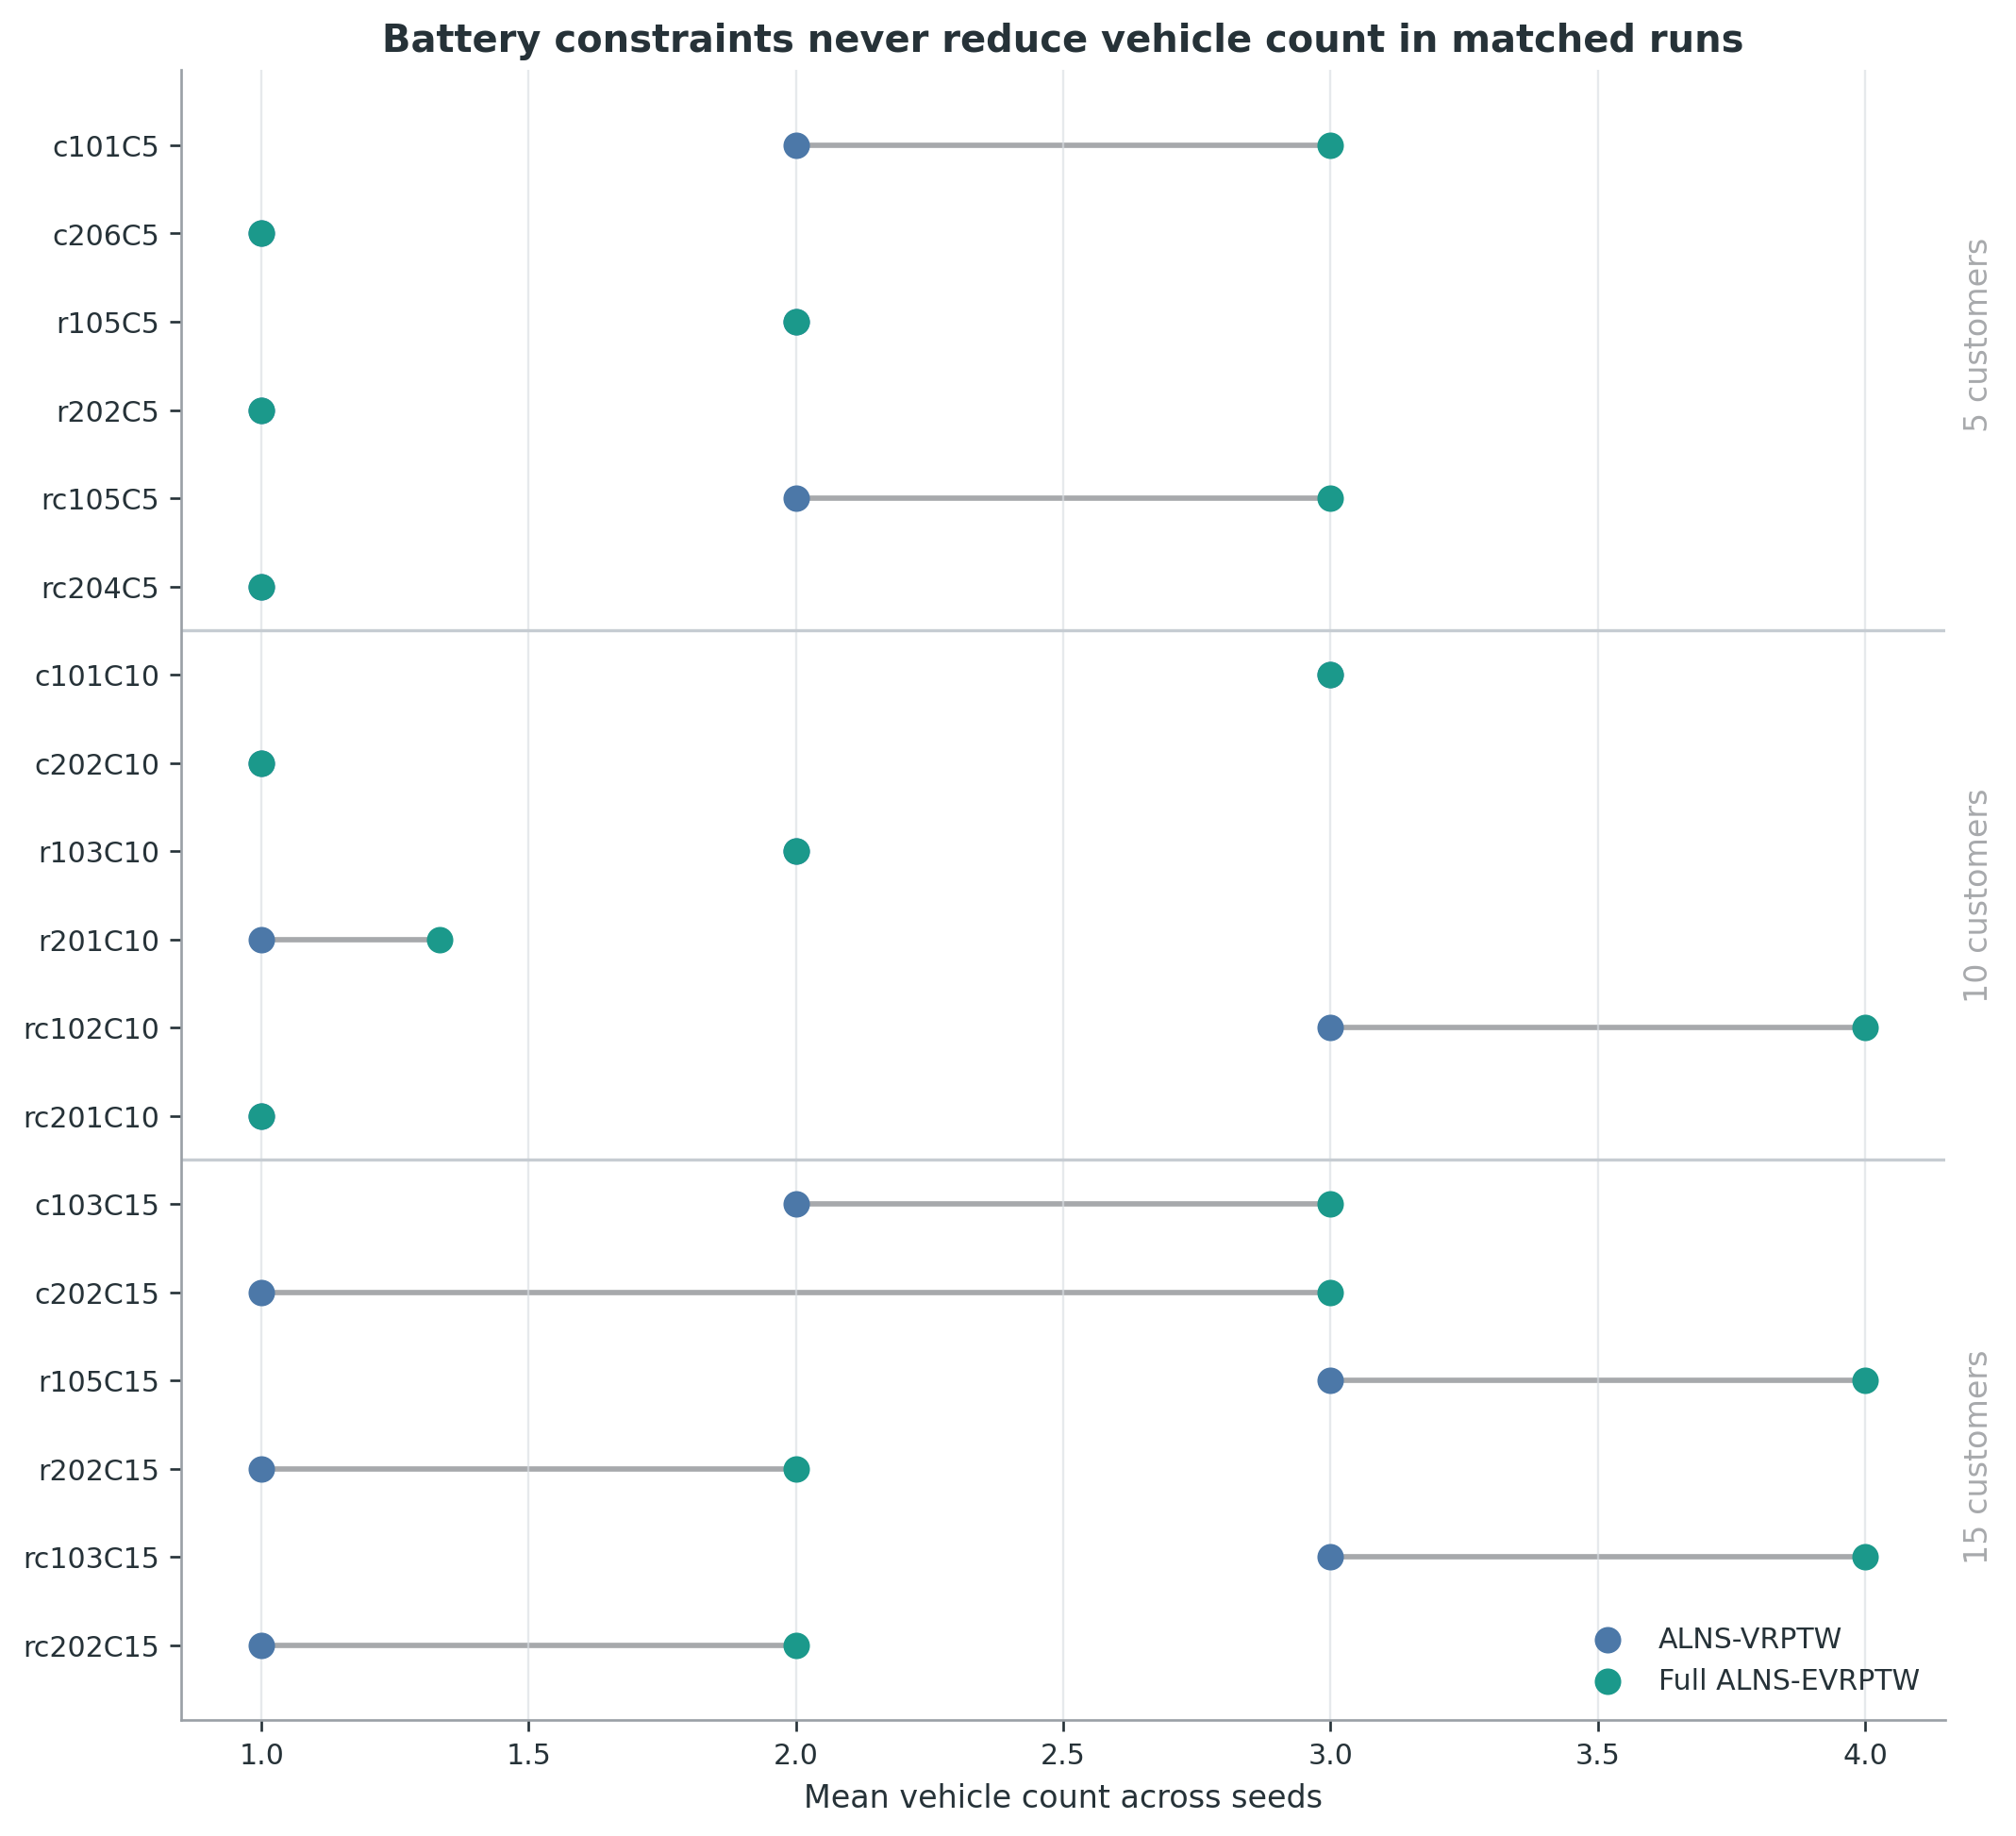
\includegraphics[width=0.84\linewidth]{fig04_vehicle_count_vr_vs_ev.png}

\vspace{-0.15cm}
{\fontsize{19}{24}\selectfont Battery constraints increased fleet size in \textbf{28/54} matched runs and never reduced it.}
\end{posterbox}

\begin{posterbox}{MAIN RESULTS}
\centering
\metric{216/216}{battery-enabled runs strictly feasible}\hfill
\metric{28/54}{matched runs used more EVs}\hfill
\metric{5.65--20.22$\times$}{runtime ratio from 5 to 15 customers}

\vspace{0.45cm}
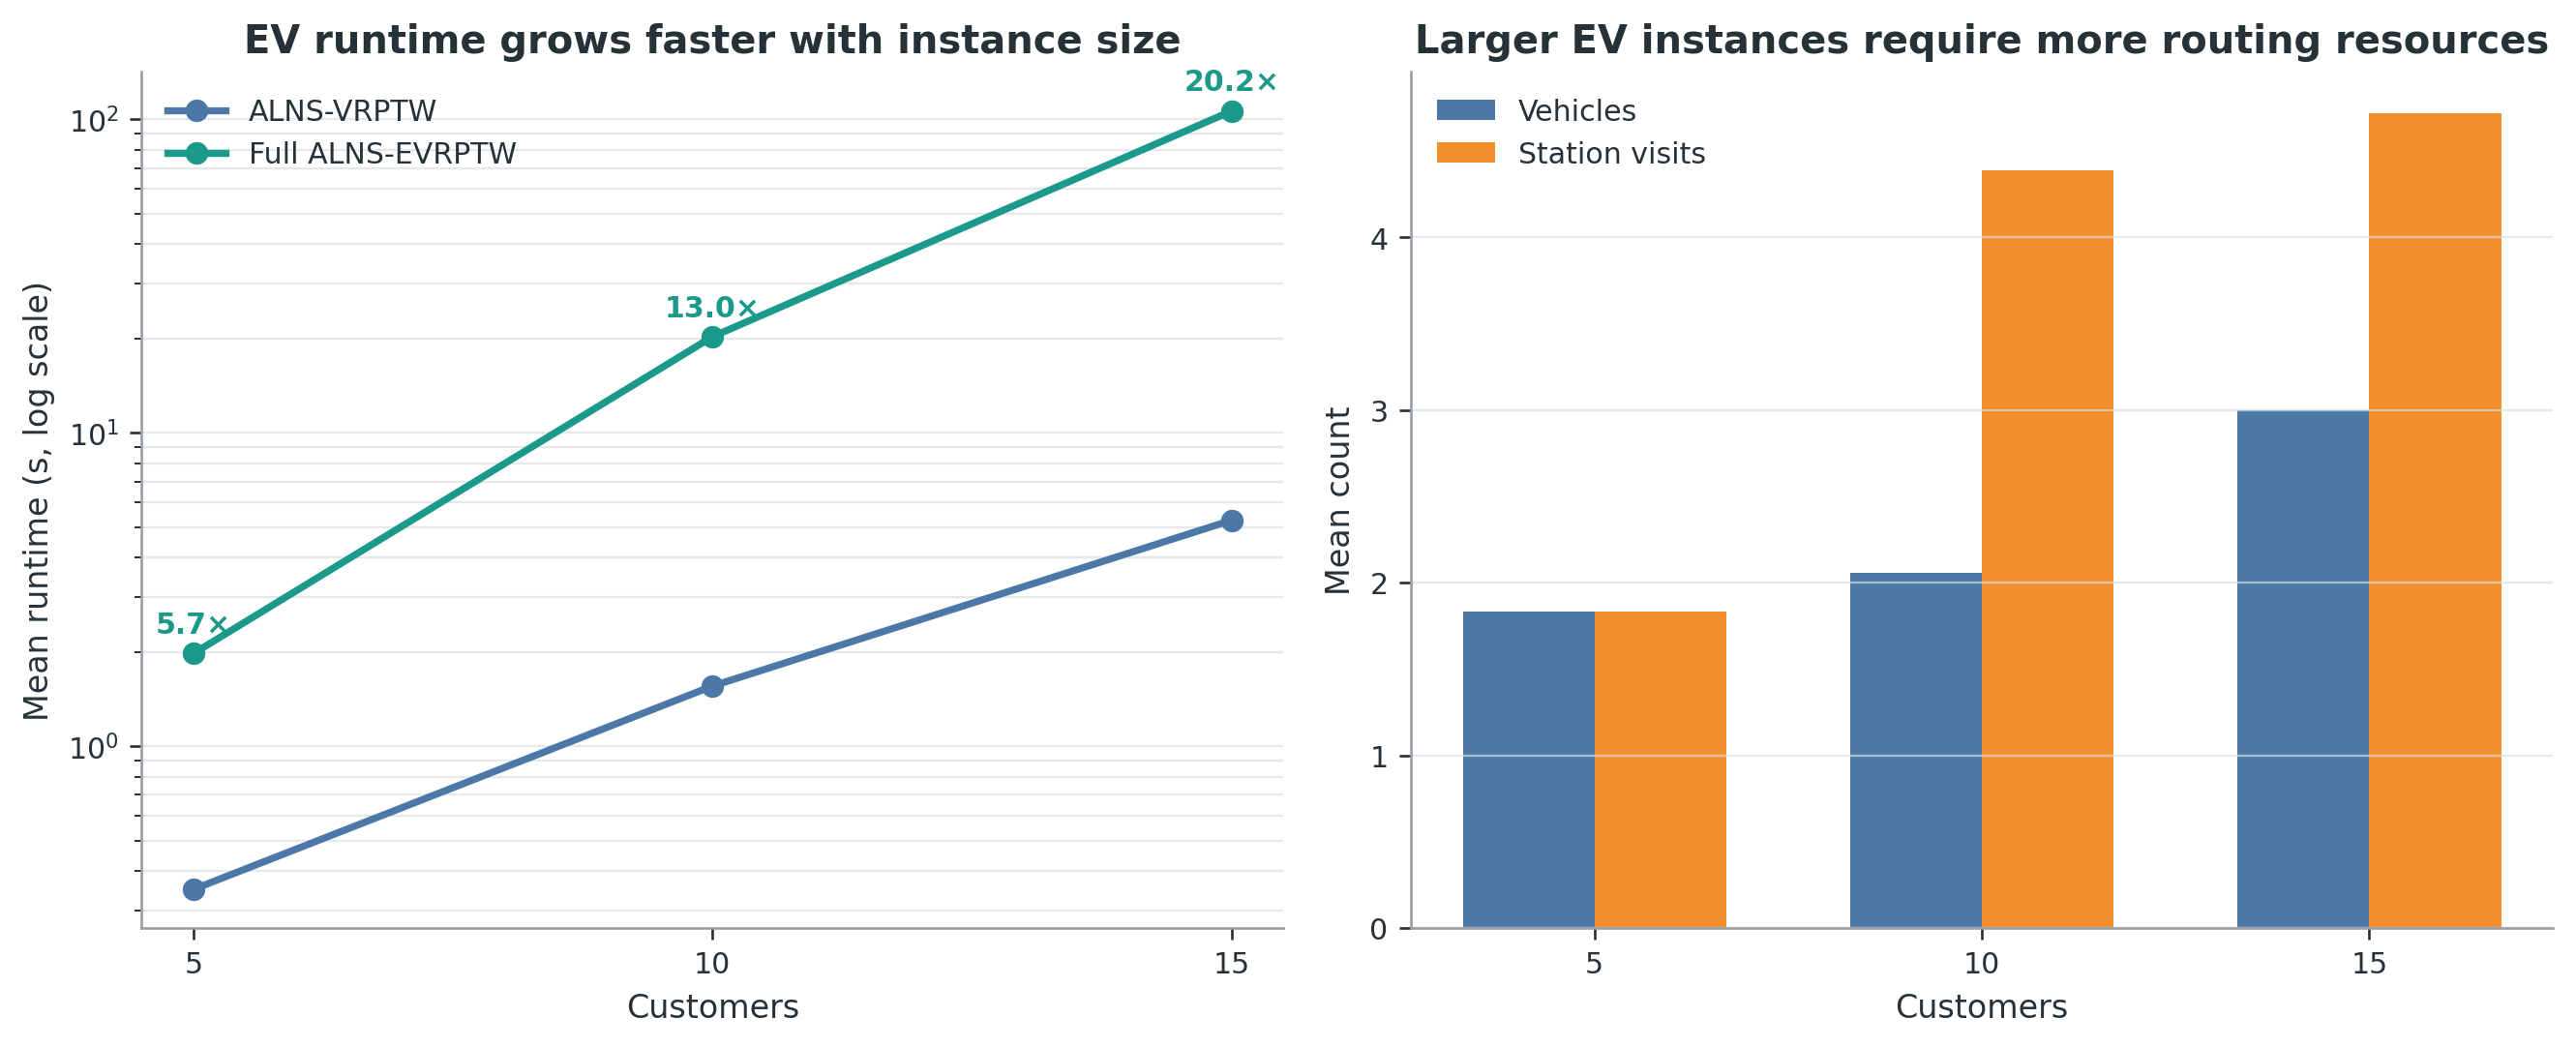
\includegraphics[width=0.95\linewidth]{fig06_scalability_and_charging.png}

\vspace{-0.1cm}
\begin{takeaway}
\fontsize{23}{29}\selectfont
Among equal-fleet comparisons, EV routes were longer in \textbf{23/26} cases, with a mean distance penalty of \textbf{+12.419}. Charging feasibility therefore raised both route length and computational cost.
\end{takeaway}
\end{posterbox}

\end{column}

\separatorcolumn

\begin{column}{\colwidth}

\begin{posterbox}{FEASIBILITY-FIRST ALNS}
\fontsize{24}{30}\selectfont
The solver uses a common destroy--repair loop for VRPTW and EVRPTW. Battery-enabled evaluation inserts charging stations greedily, propagates time and energy states, and rejects any route that remains infeasible.

\vspace{0.25cm}
\begin{itemize}
  \item \textbf{Lexicographic objective:} minimise vehicles first, then total distance.
  \item \textbf{Adaptive operators:} random, worst, and Shaw removal with greedy or regret repair.
  \item \textbf{Search control:} simulated annealing acceptance, adaptive weights, and lightweight local search.
\end{itemize}

\vspace{0.2cm}
\centering
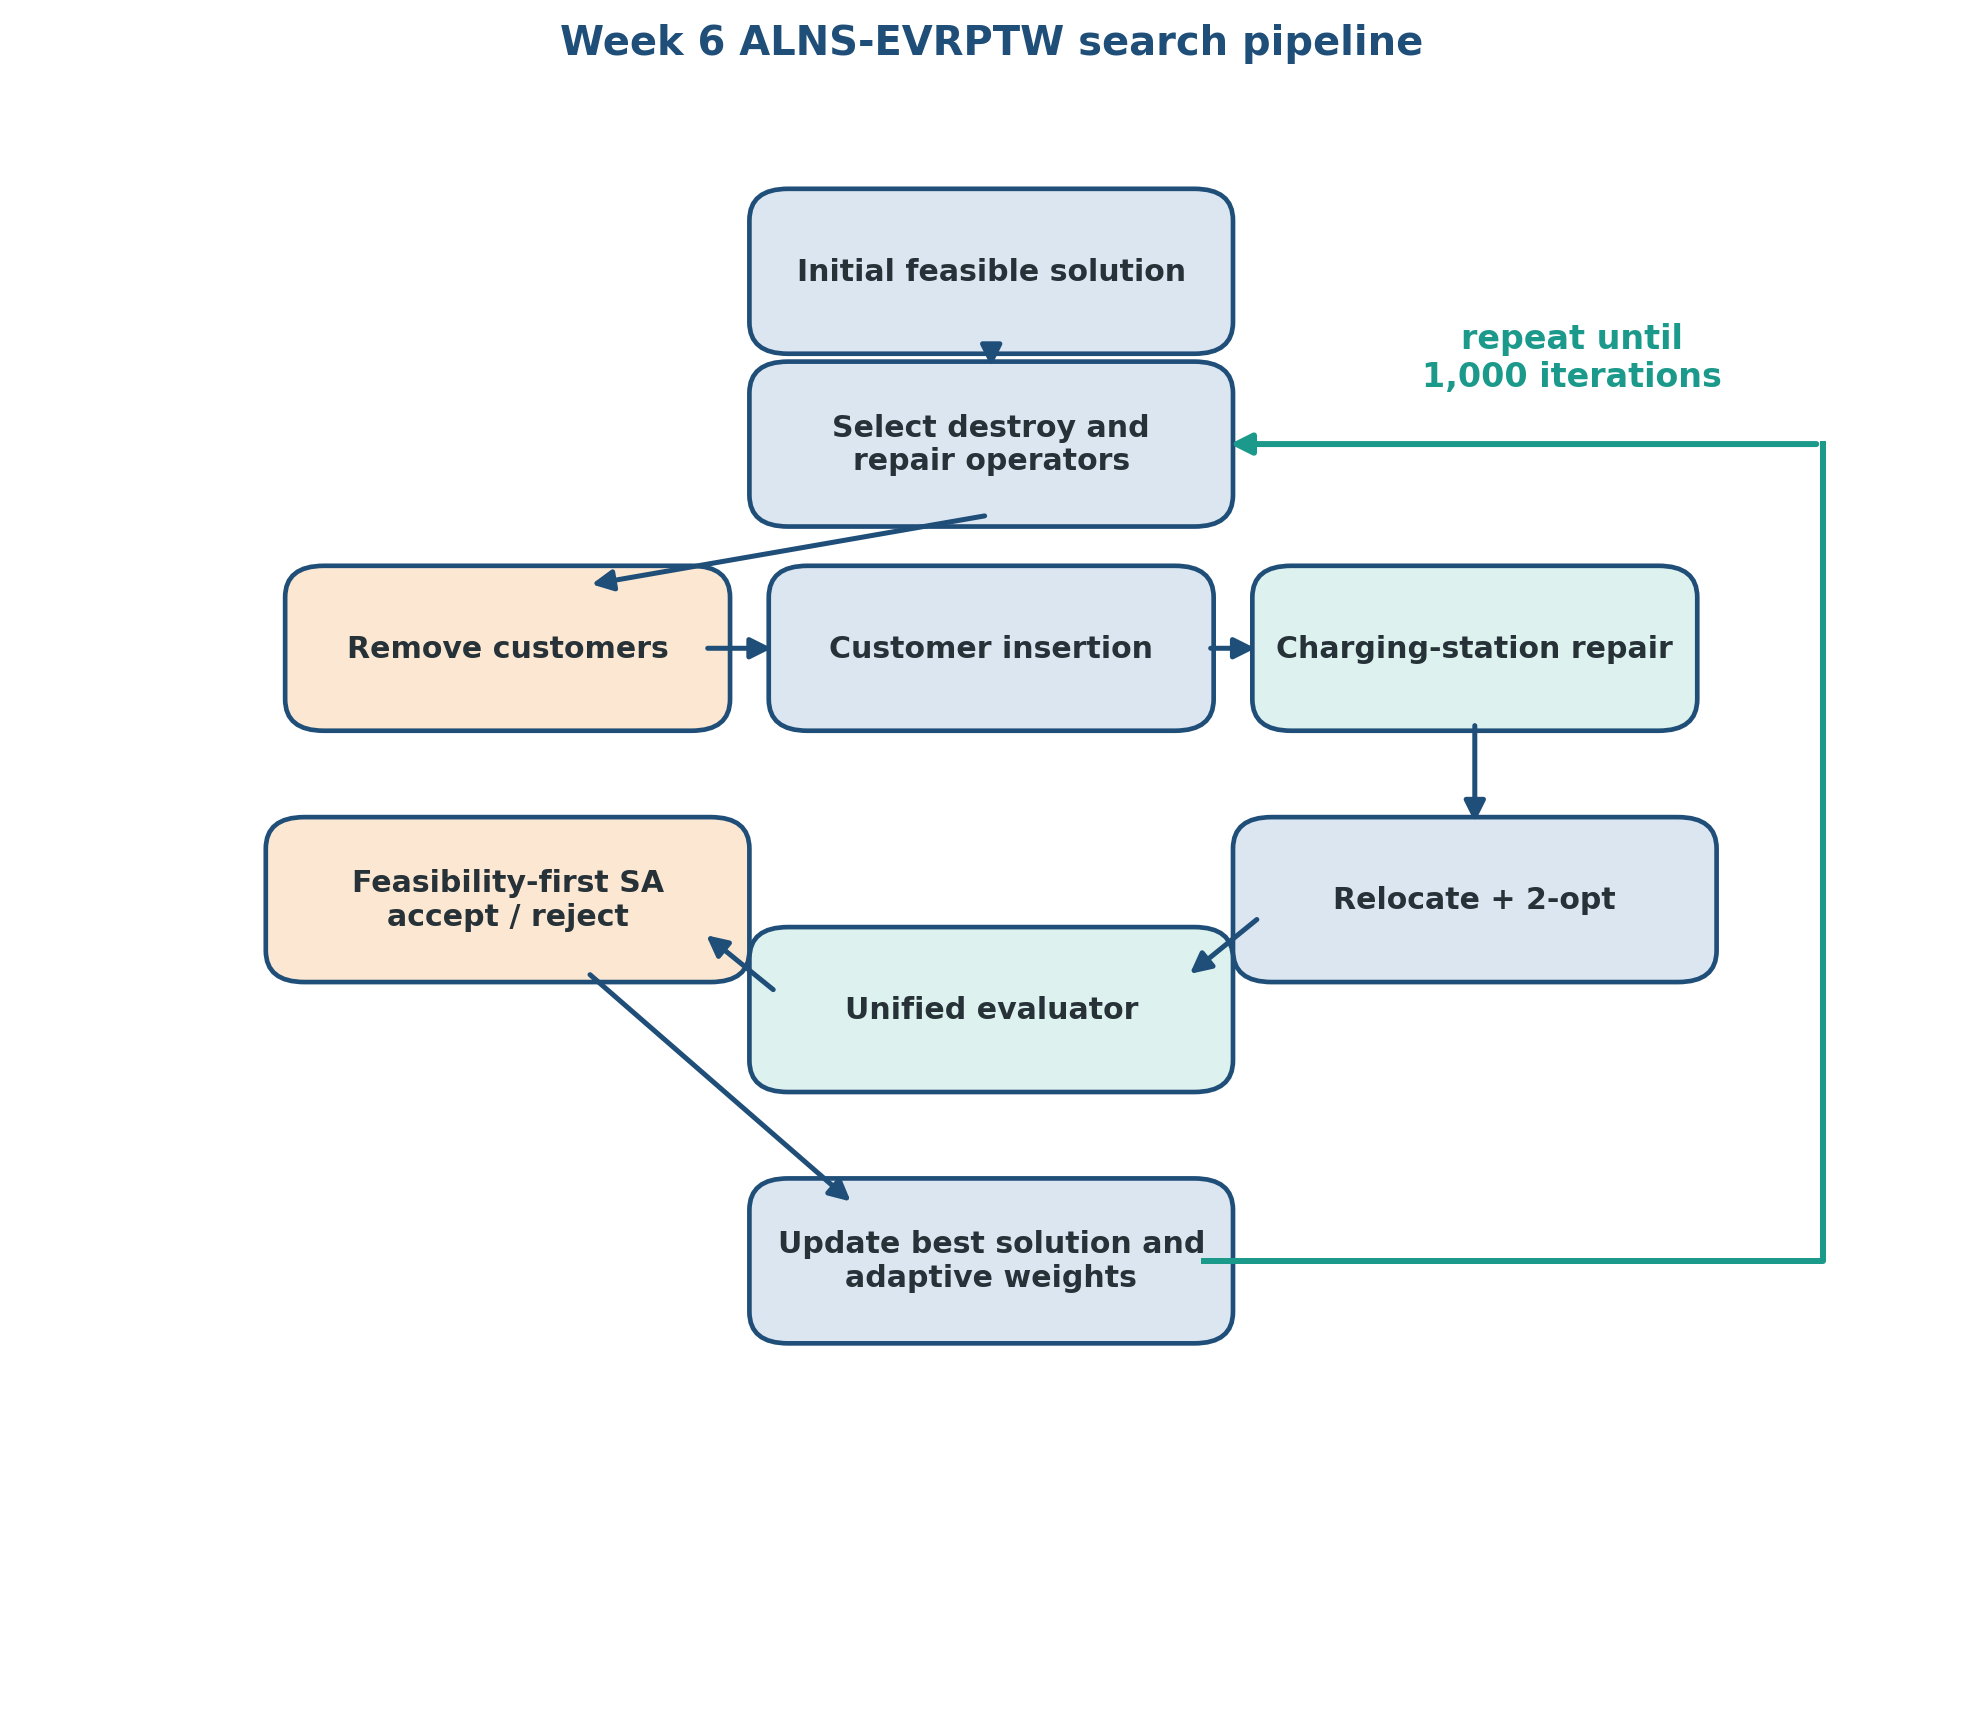
\includegraphics[width=0.91\linewidth]{fig03_alns_pipeline.png}
\end{posterbox}

\begin{posterbox}{ABLATION: WHAT DID LOCAL SEARCH ADD?}
\fontsize{23}{29}\selectfont
\centering
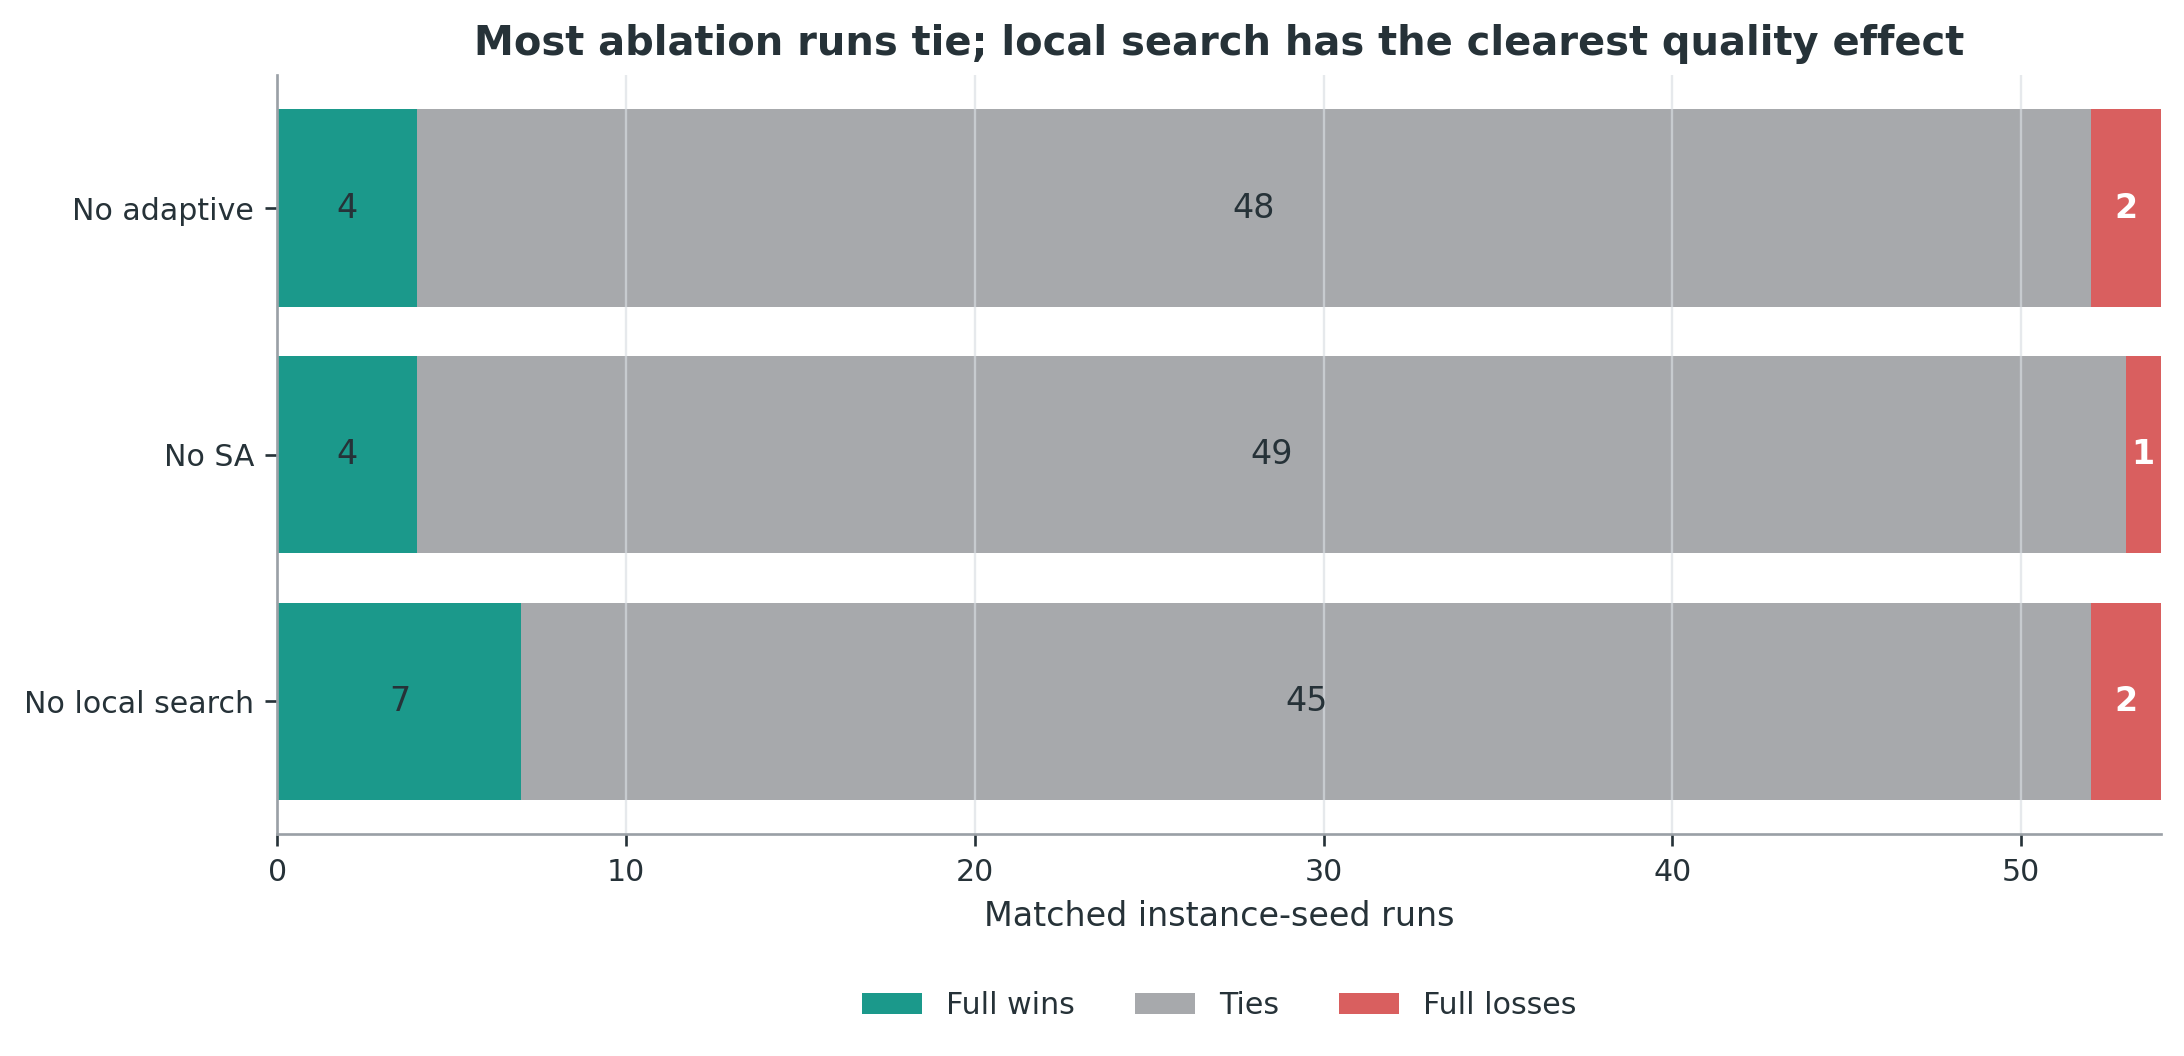
\includegraphics[width=0.95\linewidth]{fig07_ablation_win_tie_loss.png}

\vspace{0.1cm}
\begin{itemize}
  \item Full ALNS won 7, tied 45, and lost 2 of 54 paired comparisons.
  \item Removing local search reduced runtime by \textbf{47.3\%}.
  \item \textbf{95.6\%} of iterations produced equal-objective candidates, indicating limited search diversity at this budget.
\end{itemize}
\end{posterbox}

\begin{posterbox}{CONCLUSION AND LIMITATIONS}
\fontsize{24}{30}\selectfont
\begin{takeaway}
\centering\bfseries
The implementation reliably enforced strict full-recharge EV feasibility. On these small instances, electrification often required more vehicles, longer routes, and substantially more runtime.
\end{takeaway}

\vspace{0.35cm}
\textbf{Scope of the evidence}
\begin{itemize}
  \item Small benchmark subset and three seeds only.
  \item Full recharge and greedy station insertion; no station-removal move.
  \item The ablation suggests future work should target charging-specific neighbourhoods rather than more generic local search.
\end{itemize}

\vspace{0.25cm}
{\fontsize{18}{23}\selectfont
\textbf{Selected references:} Schneider et al. (2014), \emph{Transportation Science}; Pisinger and Ropke (2007), \emph{Computers \& Operations Research}.}
\end{posterbox}

\end{column}
\separatorcolumn
\end{columns}

\vspace{0.35cm}
\hspace{0.022\paperwidth}%
\begin{minipage}{0.956\paperwidth}
\begin{finalbox}
\centering
{\fontsize{30}{36}\selectfont\bfseries TAKE-HOME MESSAGE}\par
\vspace{0.45cm}
\begin{minipage}{0.30\linewidth}\centering
  {\fontsize{42}{48}\selectfont\bfseries 216/216}\par
  {\fontsize{21}{26}\selectfont strictly feasible EV runs}
\end{minipage}\hfill
\begin{minipage}{0.30\linewidth}\centering
  {\fontsize{42}{48}\selectfont\bfseries 28/54}\par
  {\fontsize{21}{26}\selectfont comparisons used more EVs}
\end{minipage}\hfill
\begin{minipage}{0.30\linewidth}\centering
  {\fontsize{42}{48}\selectfont\bfseries 47.3\%}\par
  {\fontsize{21}{26}\selectfont less runtime without local search}
\end{minipage}
\end{finalbox}
\end{minipage}
\end{frame}
\end{document}
